% !TEX program=lualatex
\RequirePackage{luatex85}
\documentclass{report}
\usepackage{geometry}
\usepackage[style=nature, citestyle=authoryear]{biblatex}
\usepackage{amsmath}
\usepackage{url}
\usepackage{graphicx}
\usepackage{tikz}
\usepackage{wrapfig}
\usepackage{booktabs}
\usepackage{tabularx}
\usepackage{multirow}
\usepackage{minted}

%drafting packages
\usepackage[doublespacing]{setspace}
\usepackage{lineno}
\usepackage{outline}

\newcommand{\titlecaption}[2]{\caption[#1]{\textbf{#1 \textbar\,} #2}}
\newcommand{\includetwo}[2]{\begin{minipage}{.45\textwidth}%
\includegraphics[width = \textwidth]{#1}%
\end{minipage}\hfill\begin{minipage}{.45\textwidth}%
\includegraphics[width = \textwidth]{#2}%
\end{minipage}}
\bibliography{ch5.bib}
\graphicspath{{./figures/}}

\begin{document}
\linenumbers

\chapter{Evaluating the impact of quality score calibration on variant calling}

\section{Introduction}
\begin{outline}
\item Brief overview of DNA sequencing; erroneous bases
	\begin{outline}
	\item DNA sequencing is a powerful tool applied in many fields of biology. Understanding how DNA and changes in DNA influence organisms and how they interact with their environment is a fundamental goal of genetics. Correctly identifying the composition of a sampled DNA molecule is therefore an important first step for many genetic studies. However, this task is not trivial; sequencing technology is inherently prone to errors which can make it difficult to discern true biological effects from technical errors. 
	\end{outline}
\item Variant calling
	\begin{outline}
	\item Because of this error, the same piece of DNA is usually sequenced multiple times to attempt to get multiple measurements and a model is applied to infer the sample genotype. While a few sequencing errors do not impede accurate inference of the genotype of a monoploid sample, sequencing errors can be difficult to distinguish from heterozygosity in diploid organisms. This problem is even more difficult for samples with higher ploidy. However, using a statistical model enables a systematic approach to genotyping every site in the genome.
	\item Additionally, a model allows the incorporation of auxiliary information when deciding the genotype at a site in a sample. For example, variant calling models often incorporate population genetic parameters that can help distinguish between sequencing errors and biological variation. The expected heterozygosity parameter \theta is particularly important;
	\end{outline}
	\item Talk about how MAQ improved variant calls by integrating alignment error, so improving base quality should also lead to improved variant calls.
\item Quality scores, Base Quality Score Recalibration, and quality score binning
\end{outline}

\section{Methods}
\begin{outline}
\item I simulated datsets with various recalibration quality using GATK's BaseQualityRecalibrator \parencite{auwera_fastq_2013}, but with variable site sets that were artificially crafted to have different false positive and false negative calls, from 0 to 100 in steps of 20. The false positive rate of 100\% produced no output except in the case of 0\% false negative rate, which produced fewer calls than any other set. All datasets containing a 100\% false positive rate were therefore discarded.
\item This produced calibrations such that the higher the false negative and false positive rate, the less well-calibrated the output reads were. Refer to Chapter \ref{ch:kbbq} for more details on how the data was simulated and the CHM1-CHM13 truth set \parencite{li_synthetic-diploid_2018}.
%new paragraph
\item I then called variants on each dataset using GATK HaplotypeCaller \parencite{poplin_scaling_2018} and evaluated the output SNP calls using RealTimeGenomics' RTG Tools vcfeval program \parencite{cleary_comparing_2015} and the truth set. I first ran the tool using the default settings, which also produces a ROC-like curve for the calls' GQ annotation. I also ran the tool using the -\phantom{}-vcf-score-field=QUAL option, which produces ROC-like curves for the site's QUAL annotation.
\item These curves are not strictly ROC curves since they plot the non-normalized number of false positives on the x-axis and the non-normalized number of true positives on the y-axis. In a true ROC plot, the false positive rate and true positive rate is plotted. However, they are similar and still show the shape of the trade-off between false positive rate and false negative rate. Since they are similar enough for the purposes of this analysis, I will refer to them as ROC plots.
\item This enabled comparison of the sensitivity and false positive rate trade-off of the two scores for each dataset. These two annotations were chosen because they represent an overall summary of the quality of the called variants.

%new paragraph
\item To evaluate the output calls, I plotted the number of false positive and true positive SNP calls for each dataset. I also constructed a heat map showing the F-measure of each dataset. This is the harmonic mean of the sensitivity and precision of the calls and is one way to summarize the accuracy of the calls.

%new paragraph
%Filter info + justifications:
%#filter: only snps
%#filter: DP > 35 & DP < 65 (+-2 SDEV from mean of ~50 assuming poisson)
%#filter: QUAL > 75; this is ~bottom 1% and the maximum F
%#   value from the previous analysis is between 75 and 150.
\item To see how filtering the calls affected their quality, I then identically filtered each variant set with two filters using bcftools view \parencite{li_sequence_2009}. The first filter is a depth filter, only accepting variants that have more than 35 aligned reads and fewer than 65. This is within two standard deviations of the mean sequencing depth of \~50, assuming the read depths are Poisson distributed. The second filter is a QUAL filter, accepting only calls with a QUAL of over 75. This threshold was chosen because it is approximately the bottom 1\% of QUAL values in each dataset and it is the lowest QUAL value that maximizes the F-measure of all the datasets. I then calculated the same statistics and made the same plots using the filtered calls.

%TODO 9/30/20: Include plots here. Run kbbq, call variants, apply filters, and compare variants from raw data.

\item Finally, I ran the kbbq software (see Chapter \ref{ch:kbbq}) with the specified genome size 605951511 and coverage 240 to recalibrate a set of reads sequenced from an individual of the non-model species \textit{Eucalyptus melliodora} \parencite{orr_phylogenomic_2020}. This dataset contains reads from 3 leaves each from 8 branches, each leaf sequenced to a depth of approximately 10X. I then called variants using HaplotypeCaller and filtered the calls using the same filters from \cite{orr_phylogenomic_2020}. At each filtering step, I recorded the number of calls that were not identical at every leaf from the same branch; these I considered false positives. I also recorded the number of calls that were not present in the final set of variants identified in \cite{orr_phylogenomic_2020}; these I considered false negatives. I then compared these values with those found in \cite{orr_phylogenomic_2020}.

\end{outline}

\section{Results}
\begin{outline}
\item To evaluate the output calls, I plotted the number of true positives and false positives for each dataset recalibrated using sets of variable sites with differing false negative and false negative rates (Figure \ref{fig:vc_fptp}). This shows that improved calibration increases the number of true positive variants called. However, improved calibration also increases the number of false positives. More detail about the relationship between false positives and negatives in the database of calibrated sites are shown in the heat maps in Figures \ref{fig:vc_fph} and \ref{fig:vc_tph}.
\end{outline}


\begin{figure}
\centering
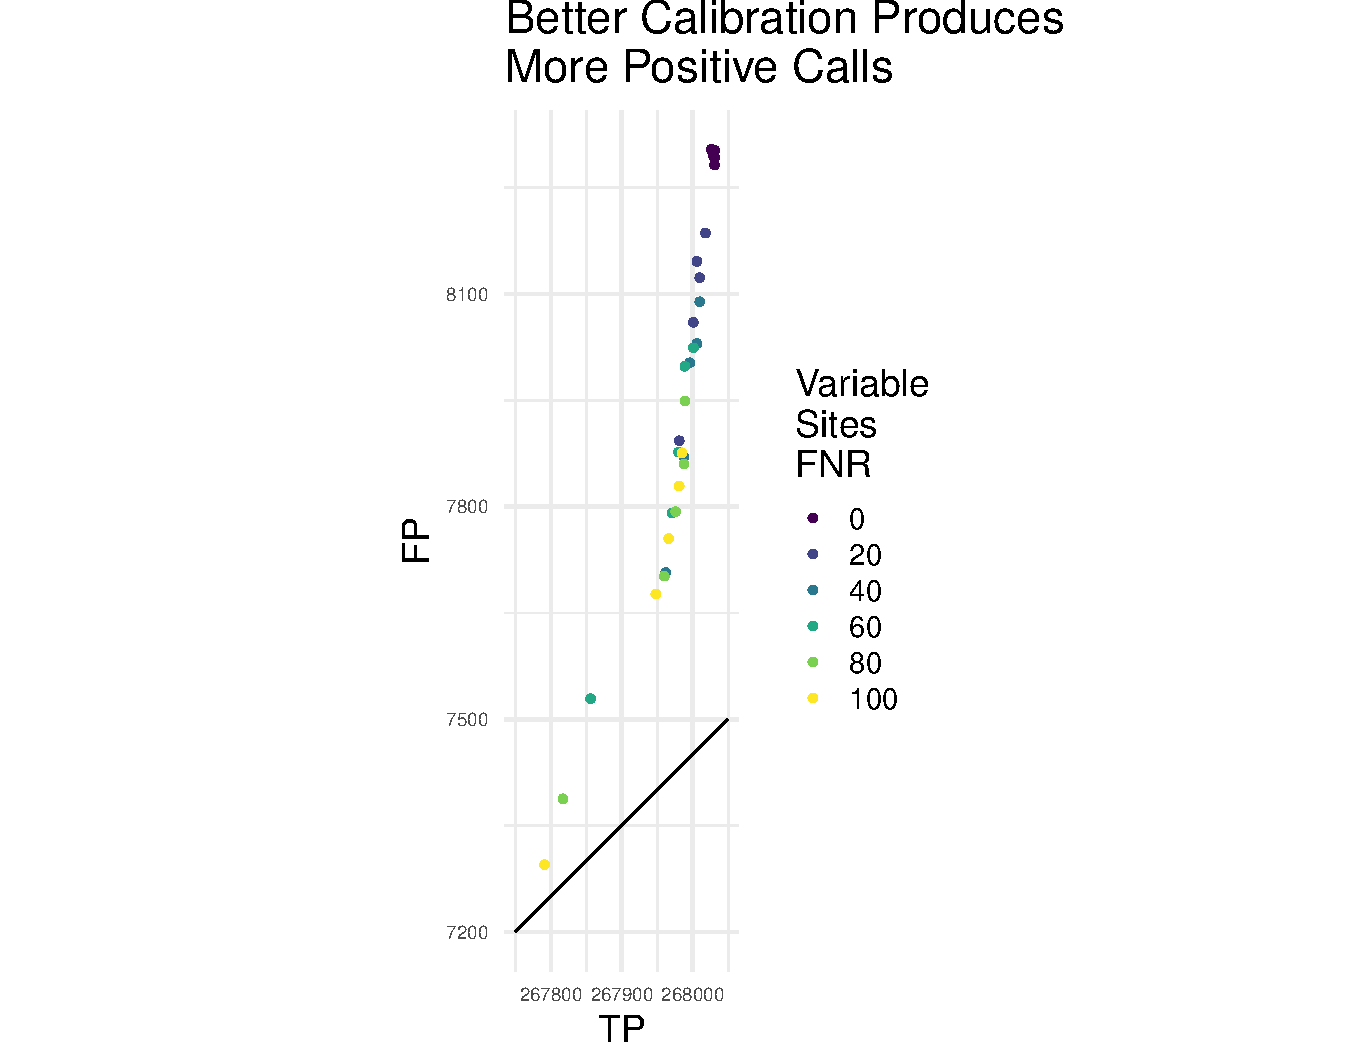
\includegraphics[width = .8\textwidth]{tp_fp_plot.pdf}
\titlecaption{Unfiltered True Positive and False Positive Calls}{The output number of positive calls for each dataset. The false negative rate of the set of variable sites used to calibrate the reads used to produce each callset is shown. As the false negative rate decreases, the number of both true positive and false positive calls increases.}
\label{fig:vc_fptp}
\end{figure}

\begin{figure}
\centering
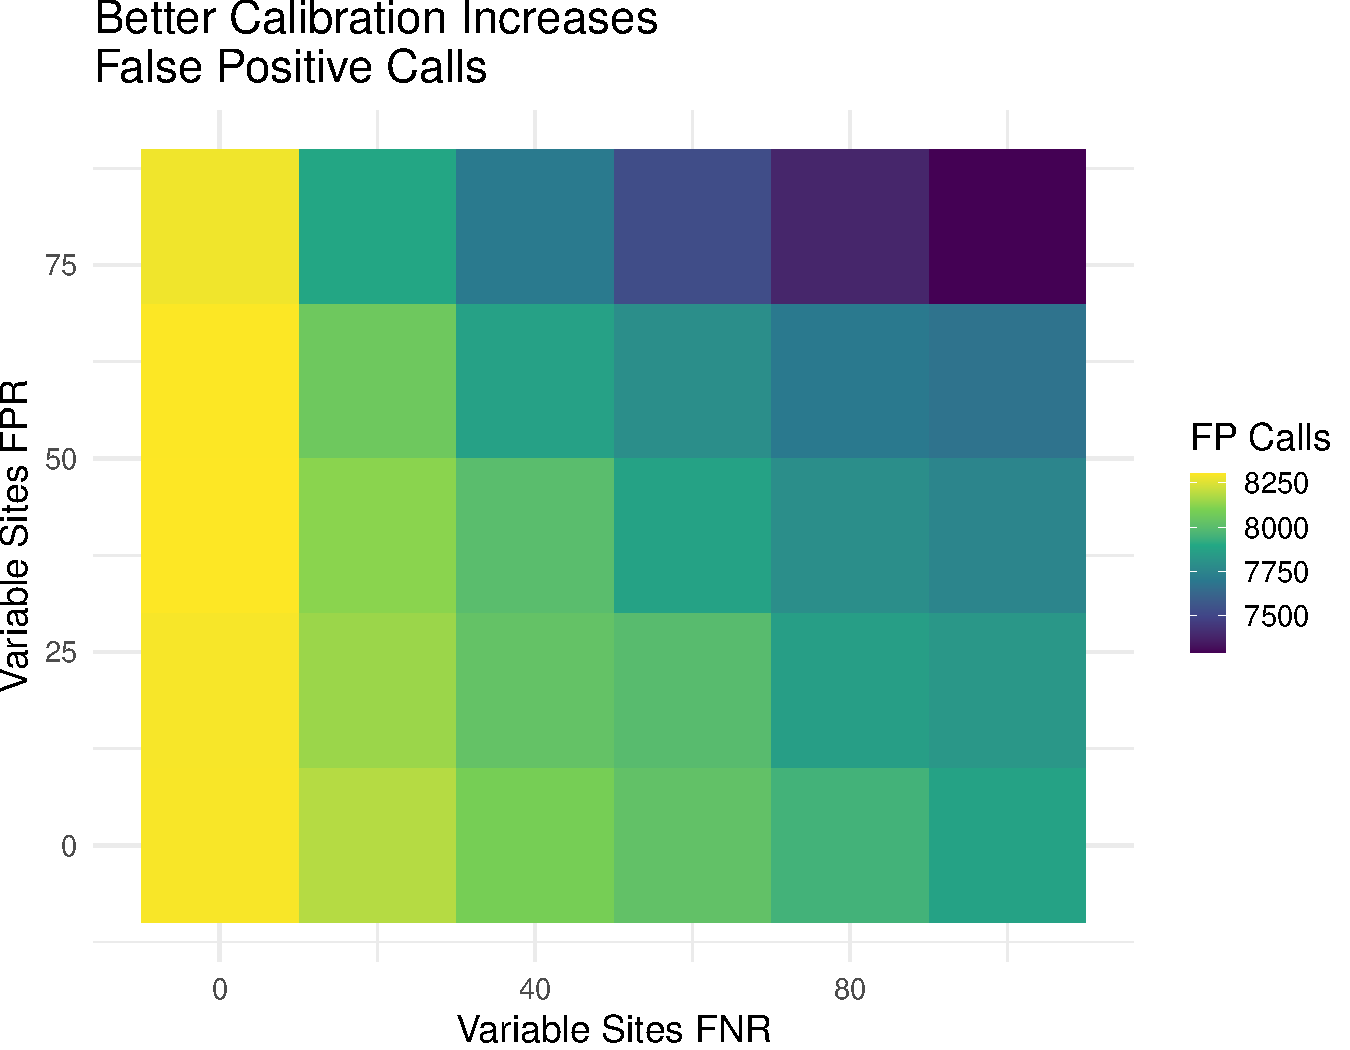
\includegraphics[width = .7\textwidth]{fp_heatmap.pdf}
\titlecaption{Unfiltered False Positives Heatmap}{The output number of false positive calls for each dataset. The false negative and false positive rate of the set of variable sites used to calibrate the input reads is shown on the x and y axis. The color of each cell represents the number of unfiltered false positive SNP calls. As the false negative and positive rates decrease, the base quality scores become more calibrated, and more calibrated data produces more false positive calls.}
\label{fig:vc_fph}
\end{figure}

\begin{figure}
\centering
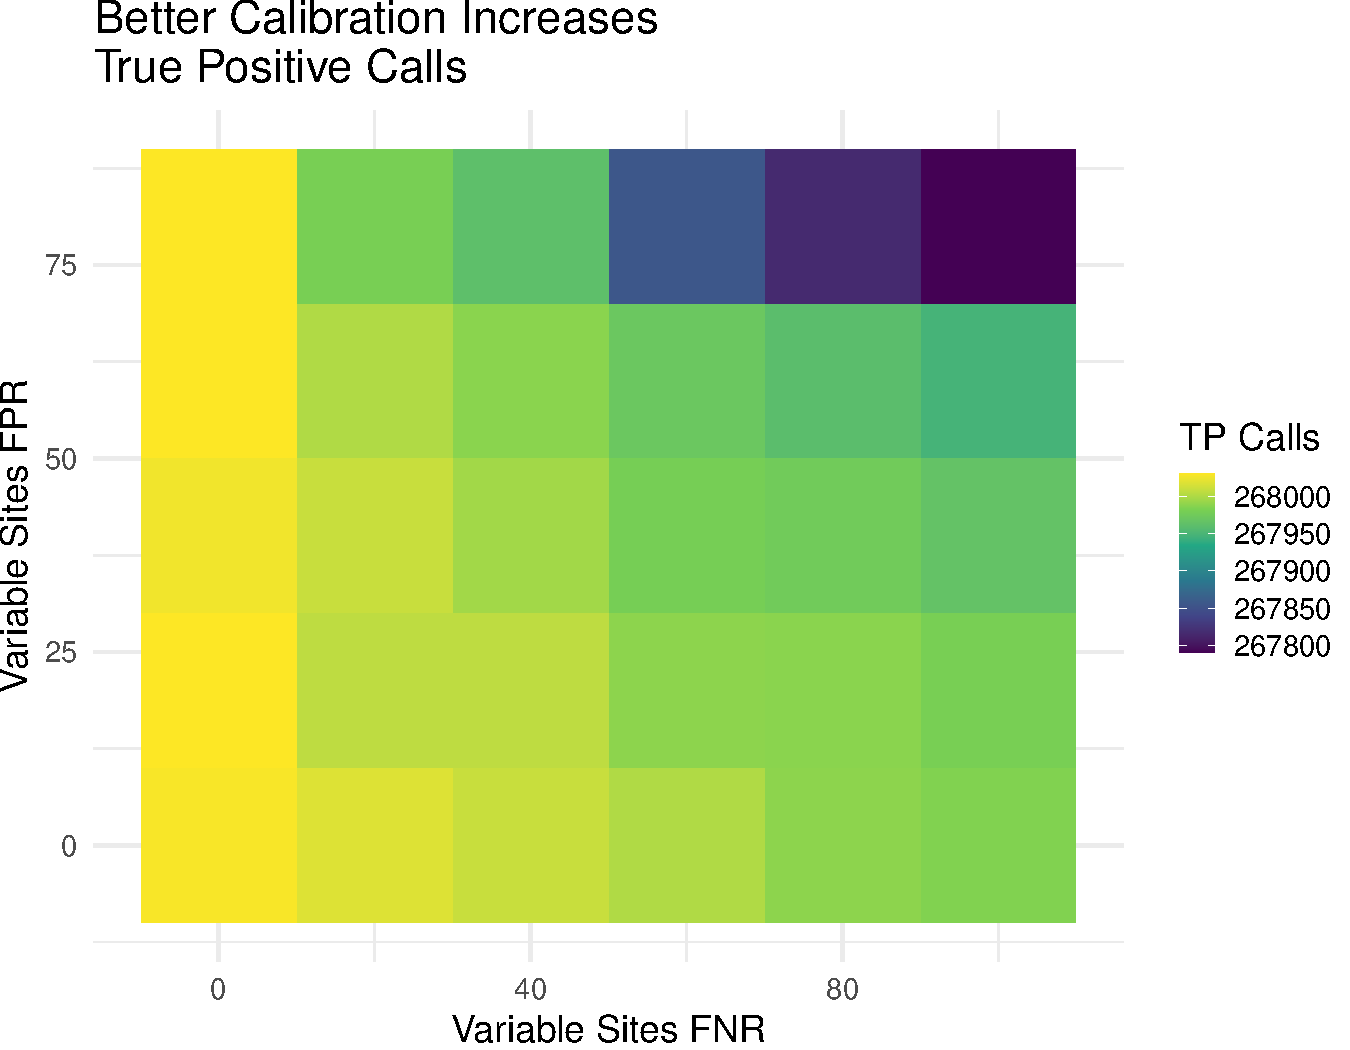
\includegraphics[width = .7\textwidth]{tp_heatmap.pdf}
\titlecaption{Unfiltered True Positives Heatmap}{The output number of true positive calls for each dataset. The false negative and false positive rate of the set of variable sites used to calibrate the input reads is shown on the x and y axis. The color of each cell represents the number of unfiltered false positive SNP calls. As the false negative and positive rates decrease, the base quality scores become more calibrated, and more calibrated data produces more true positive calls.}
\label{fig:vc_tph}
\end{figure}

\begin{outline}
\item To determine the impact of these variants on the overall quality of the callsets, I also plotted the sensitivity and precision of each dataset (Figures \ref{fig:vc_sens} and \ref{fig:vc_prec}). As the data become more well-calibrated, the sensitivity of the caller increases; however, the precision of the caller also increases. This means that the caller is able to detect more true variants, but a higher proportion of the calls it makes are false positives. To visualize the trade-off between sensitivity and precision, I plotted the precision against the sensitivity of each dataset, shown in Figure \ref{fig:vc_sens_prec}. To summarize the overall effect on accuracy, I show how the F-statistic changes across each dataset in Figure \ref{fig:vc_f_heatmap}.
\end{outline}


\begin{figure}
\centering
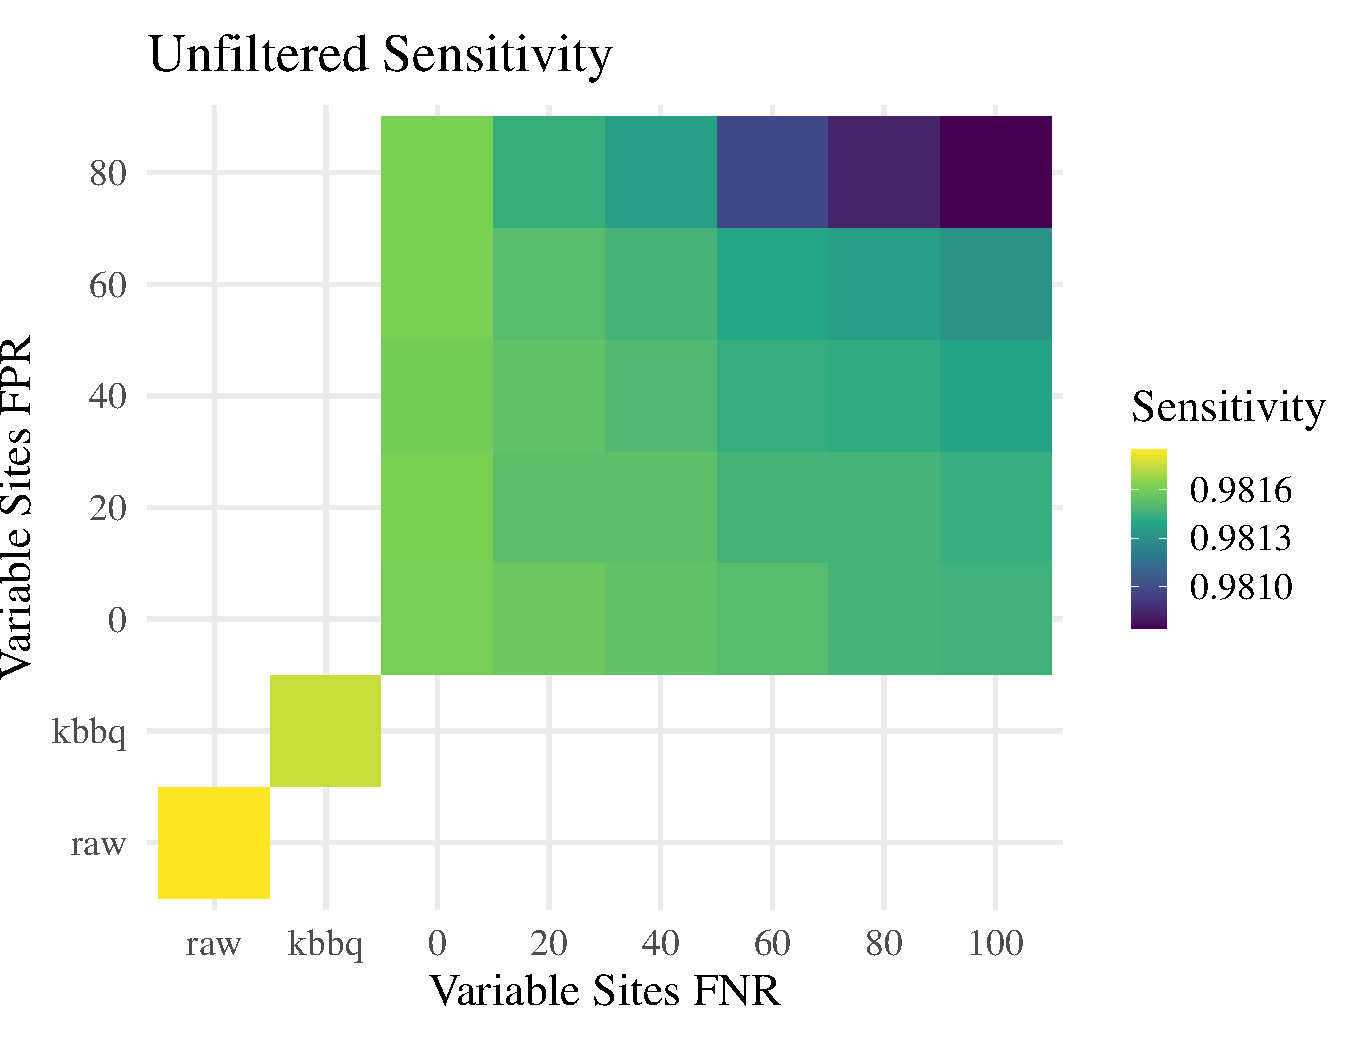
\includegraphics[width = .7\textwidth]{sensitivity.pdf}
\titlecaption{Unfiltered Sensitivity Heatmap}{The sensitivity of the variant caller on each dataset with no filtering. As the base quality score calibration of the input reads increases, the sensitivity of the caller increases.}
\label{fig:vc_sens}
\end{figure}

\begin{figure}
\centering
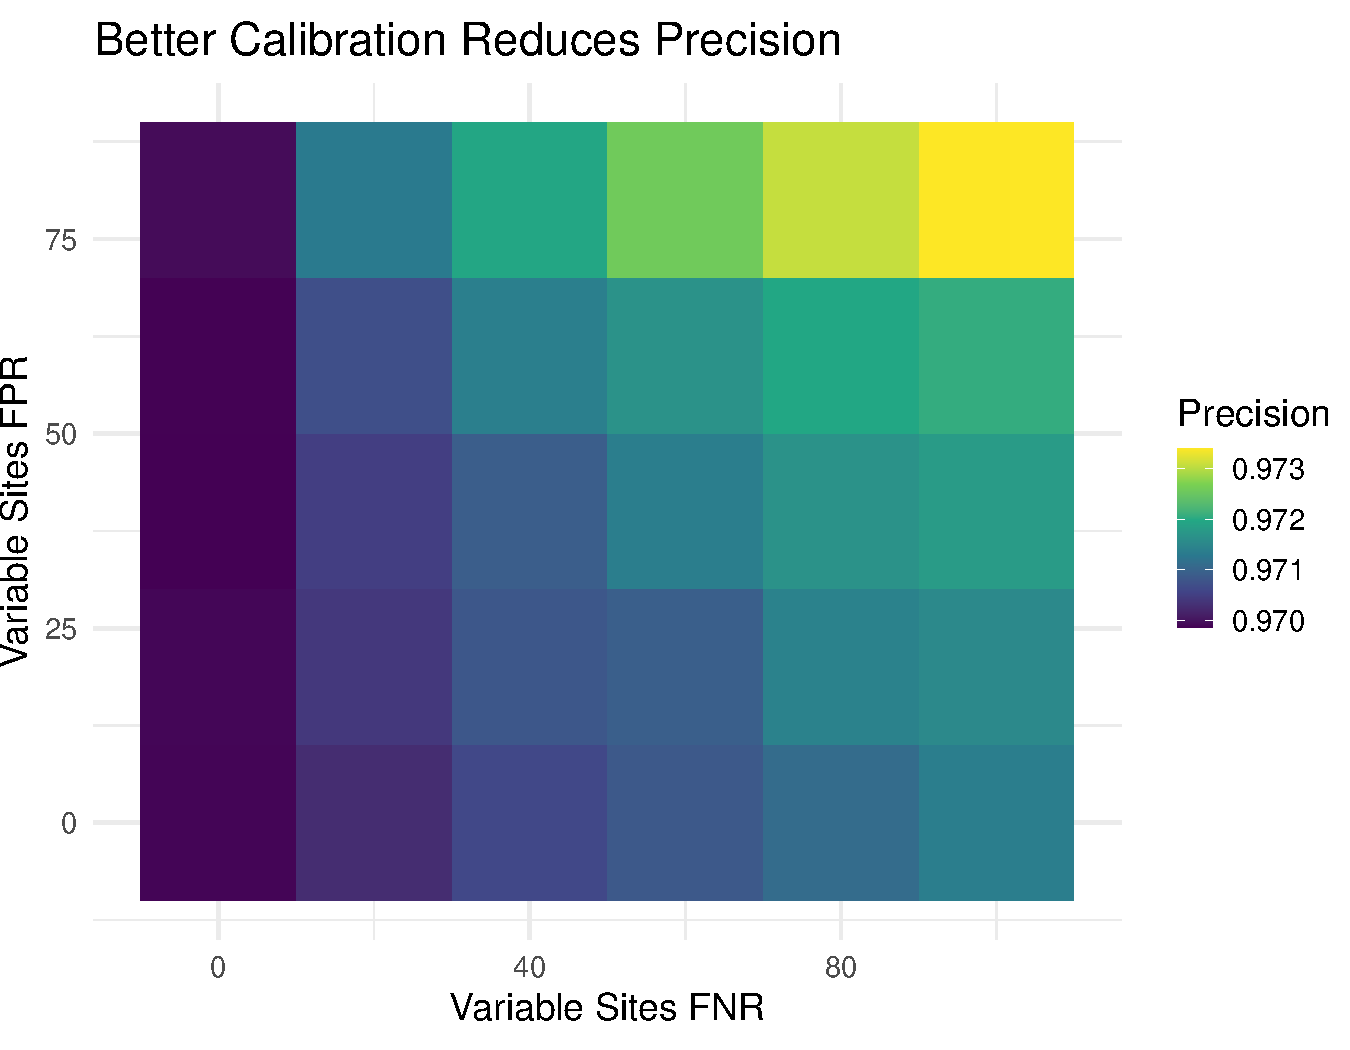
\includegraphics[width = .7\textwidth]{precision.pdf}
\titlecaption{Unfiltered Precision Heatmap}{The precision of the variant caller on each dataset with no filtering. As the base quality score calibration of the input reads increases, the precision of the caller decreases.}
\label{fig:vc_prec}
\end{figure}

\begin{figure}
\centering
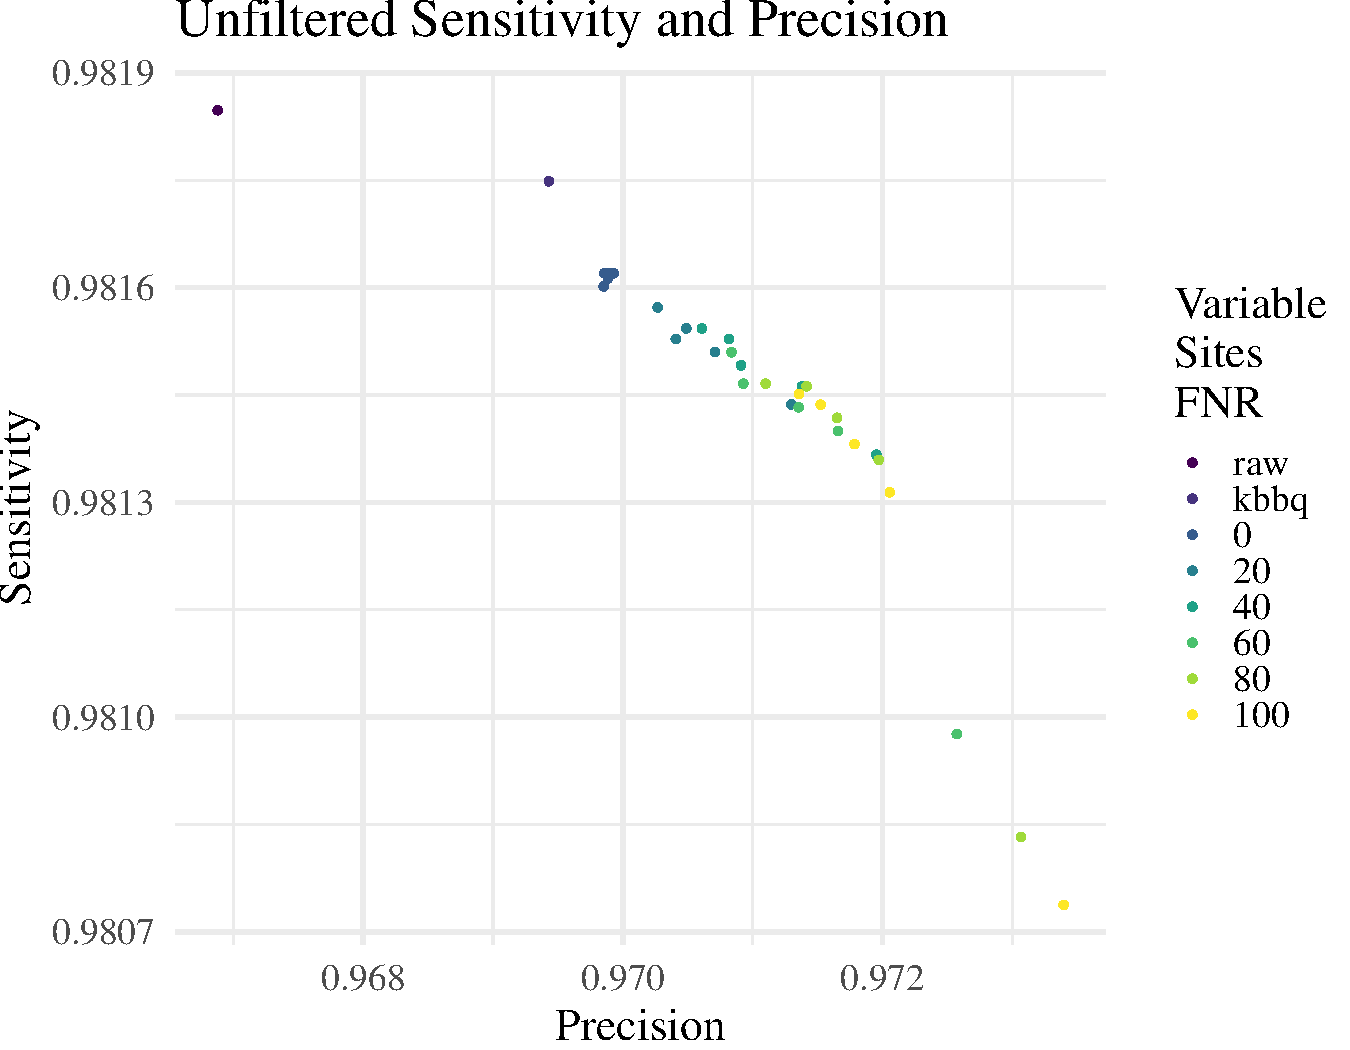
\includegraphics[width = .8\textwidth]{sens_precision.pdf}
\titlecaption{Sensitivity and Precision of Unfiltered Calls}{The sensitivity and precision of the variant caller on each dataset with no filtering. As the base quality score calibration of the input reads increases, the sensitivity of the caller increases but the precision of the caller decreases.}
\label{fig:vc_sens_prec}
\end{figure}

\begin{figure}
\centering
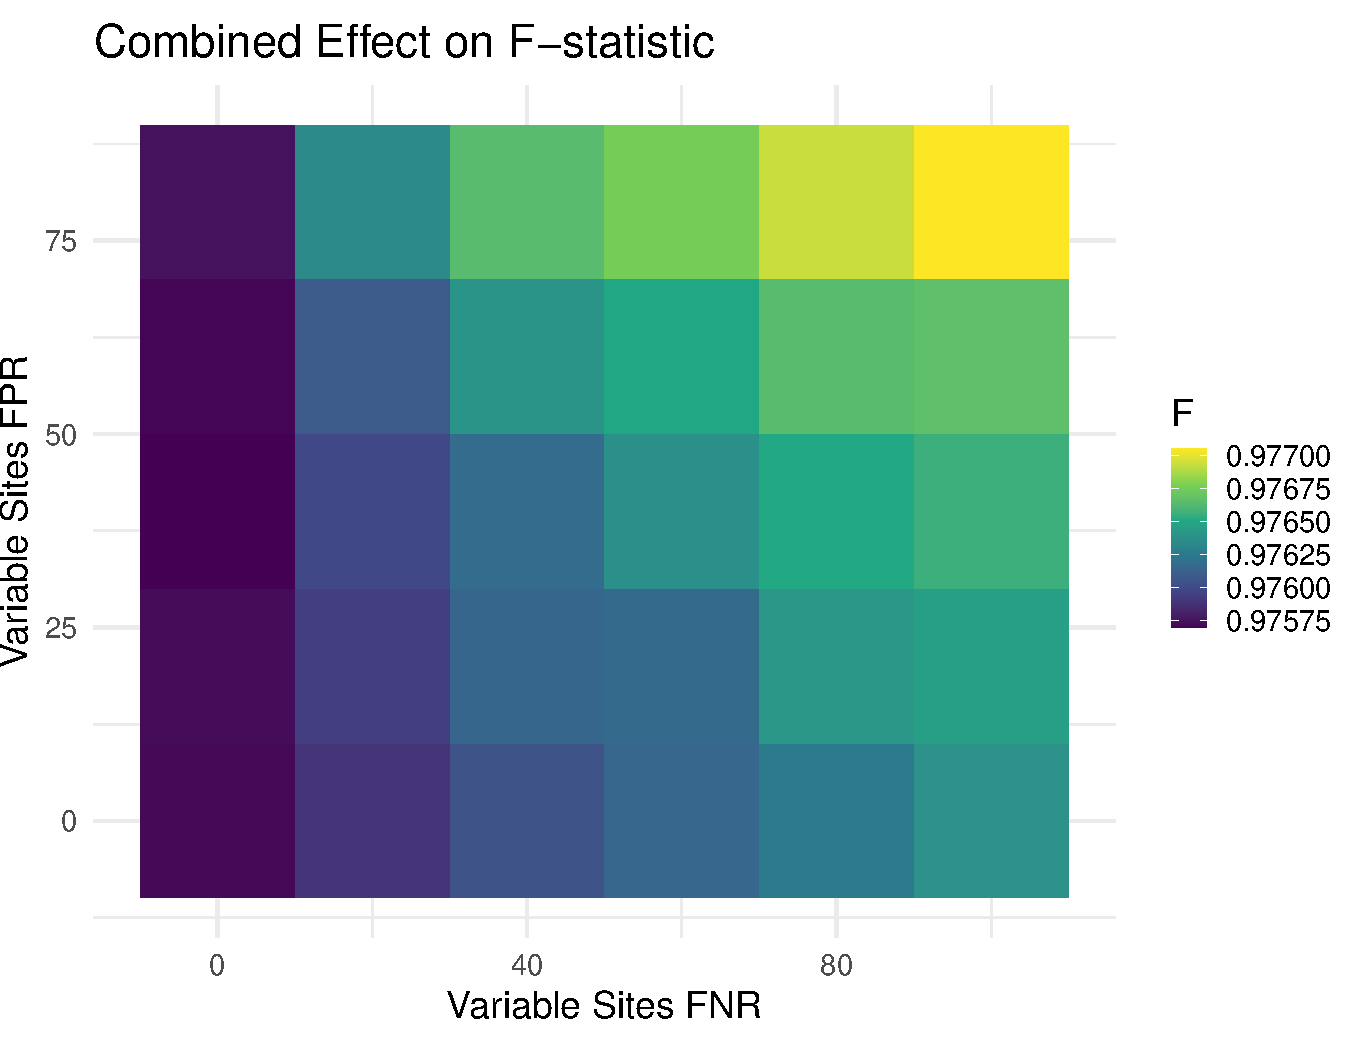
\includegraphics[width = .8\textwidth]{f_heatmap.pdf}
\titlecaption{F-measure of Unfiltered Calls}{The F-measure of the unfiltered calls of each dataset. As the base quality score calibration of the input reads increases, the F-measure of the caller decreases. This is driven by the fact that the increase in sensitivity of the caller is much smaller than the decrease in precision.}
\label{fig:vc_f_heatmap}
\end{figure}

\begin{outline}
\item Since the base quality score of the reads used to support each genotype call evidently play a role in whether to emit a variant, I wanted to see how the differences in calibration affected the annotations output by the caller. To that end, I plotted a ROC-like curve showing how the number of false positive and false negative calls for variants filtered according to the QUAL (Figure \ref{fig:vc_qualroc}) and GQ (Figure \ref{fig:vcf_gqroc}) annotations. These are both statistics that summarize the quality of the emitted site in a single, increasing score, and so are well-suited for ROC analysis. According to the VCF standard, the QUAL score is a phred-scaled probability that the ALT allele(s) present in the call are not actually present, $P($ALT is wrong$)$. The GQ score is the phred-scaled conditional probability the genotype call is incorrect given the site is variable, $P($genotype is wrong $|$ site is variant$)$.
\end{outline}


\begin{figure}
\centering
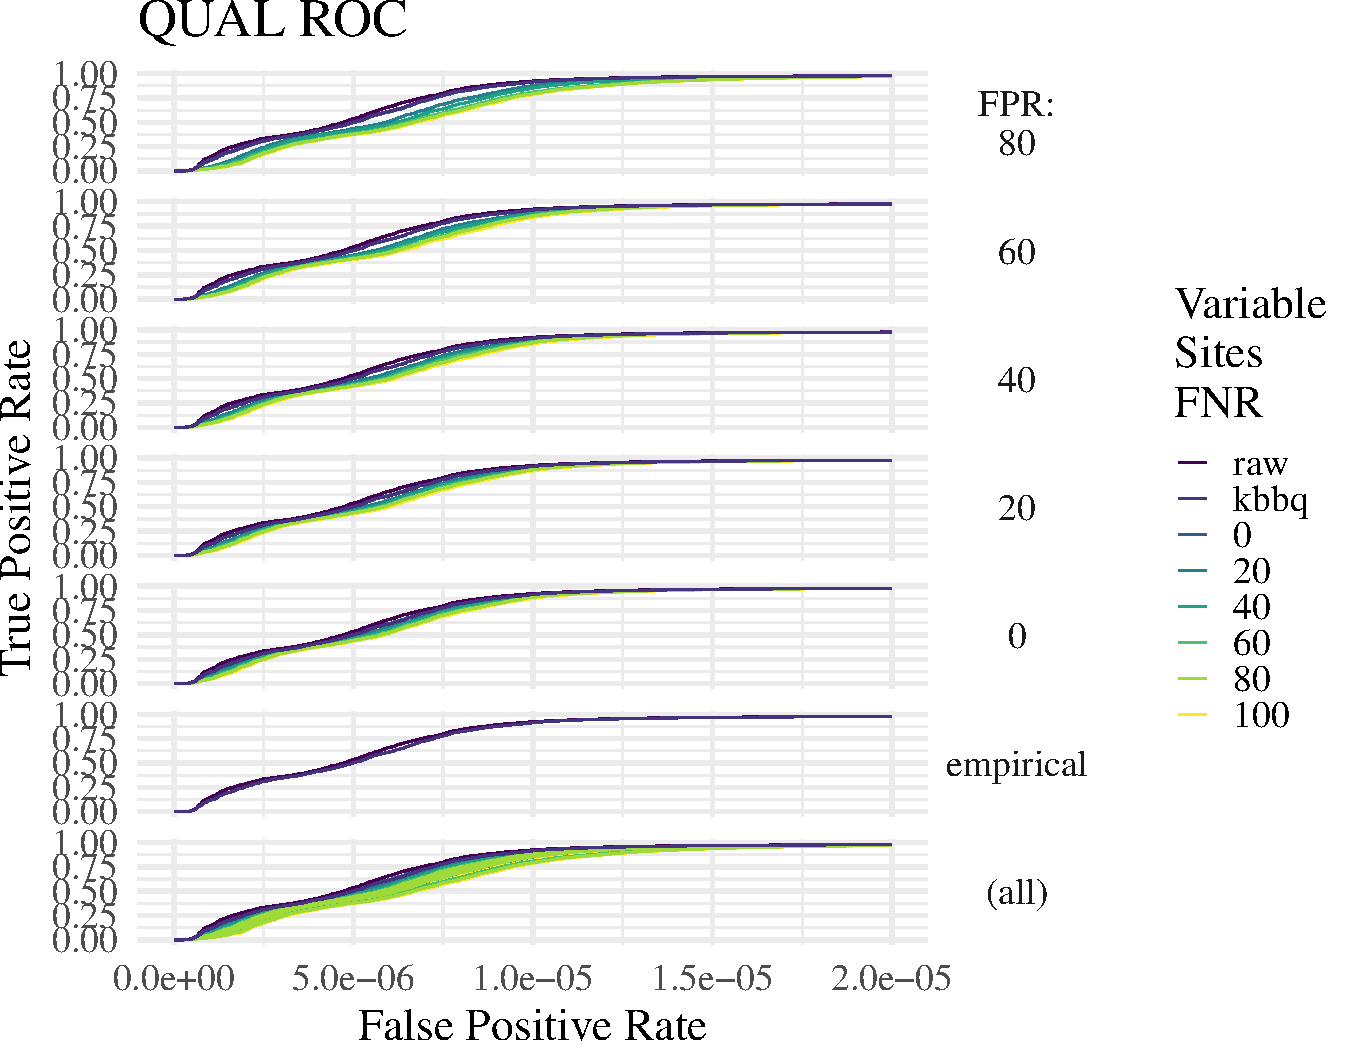
\includegraphics[width=.7\textwidth]{qualroc.pdf}
\titlecaption{Unfiltered QUAL ROC Curve}{The ROC curve for the QUAL score of an output call for the unfiltered calls of each dataset. The color of each line represents the false negative rate of the set of variant sites used as input to recalibrate the reads used to call variants. Each point in the line represents the number of false positive and false negative calls that have a score above the QUAL threshold for that point. As this threshold decreases, the number of false positives and true positives increases, though at different rates. These plots show that as the false positive rate increases, the number of true positive calls increases at a faster rate for the well-calibrated data than in other datasets.}
\label{fig:vc_qualroc}
\end{figure}

\begin{figure}
\centering
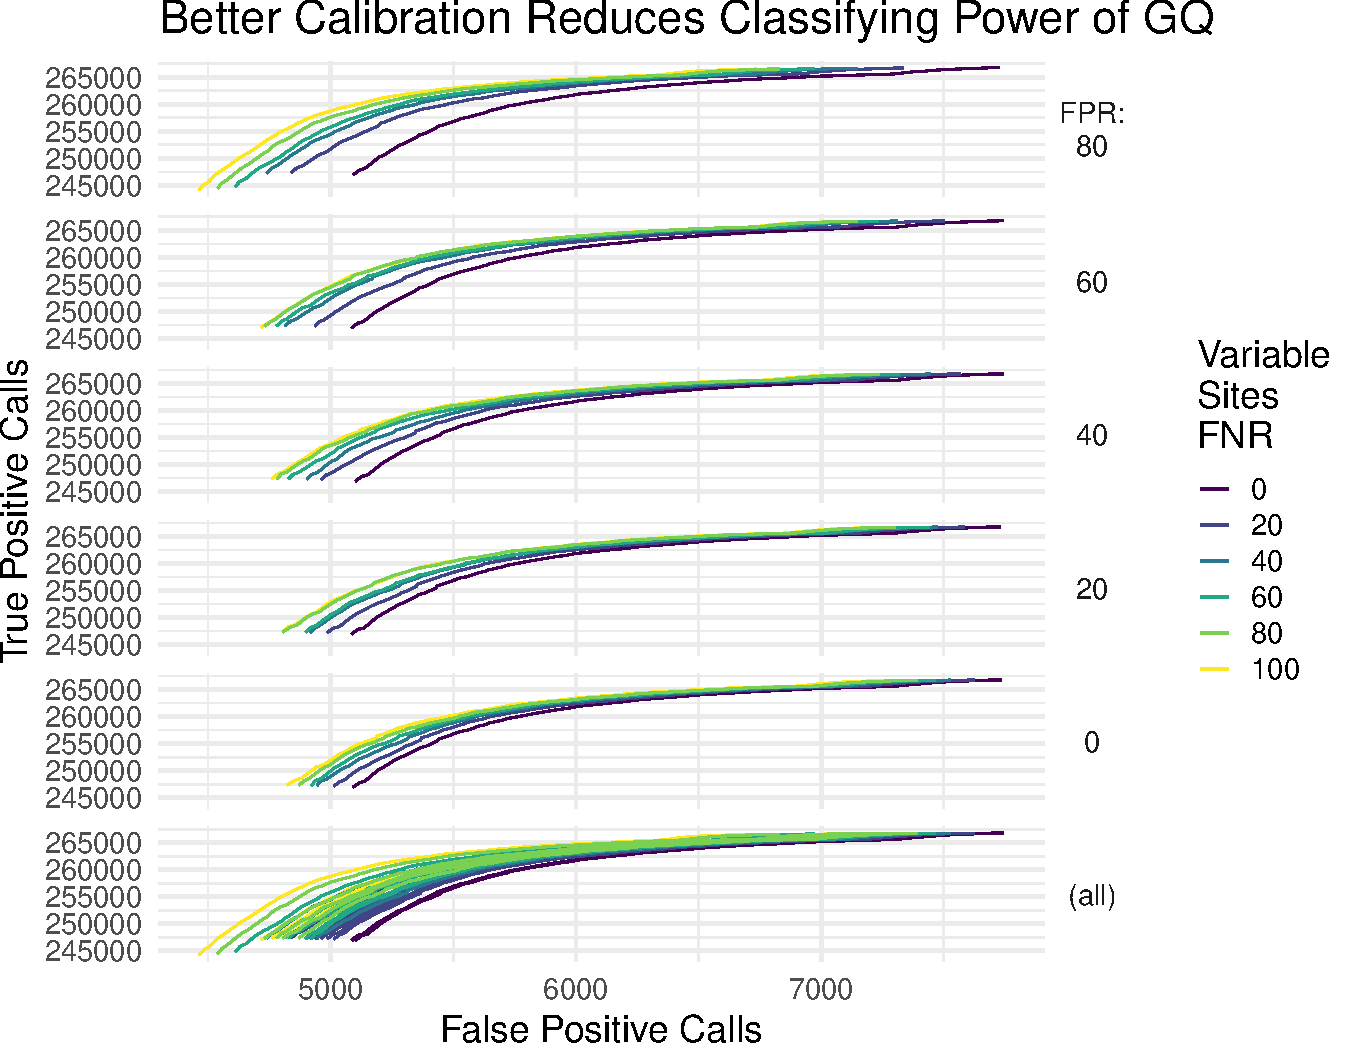
\includegraphics[width=.7\textwidth]{gqroc.pdf}
\titlecaption{Unfiltered GQ ROC Curve}{The ROC curve for the GQ score of an output call for the unfiltered calls of each dataset. The color of each line represents the false negative rate of the set of variant sites used as input to recalibrate the reads used to call variants. Each point in the line represents the number of false positive and false negative calls that have a score above the GQ threshold for that point. As this threshold decreases, the number of false positives and true positives increases, though at different rates. These plots show that as the false positive rate increases, the number of true positive calls increases at a lower rate for the well-calibrated data than in other datasets.}
\label{fig:vc_qualroc}
\end{figure}

\begin{outline}
\item As the ROC plots show that each dataset would respond to filtering differently, I examined how the calls would improve or not after filtration. Since the ROC curves show each dataset would respond differently to a QUAL filter, I used a small QUAL filter filtering out variants with the lower 1\% of QUAL scores. This percentage coincides with the smallest QUAL value of the QUAL values that maximize the F-measure of every dataset. These values are shown in Figure \ref{fig:vc_f_heatmap}. Depth filters are very common after variant calling, so I also used a depth filter to filter out calls that had unusually high or low depth.
\item This resulted in a similar pattern of positive calls as the unfiltered data, seen in Figure \ref{fig:vc_flt_p}; better calibrated data had more false positive and true positive calls. However, the difference between the best-calibrated data and worst-calibrated was much larger after filtration. Additionally, the difference between the number of true positives in the best-calibrated data and the next-best calibration at each step was smaller. So filtering caused even imperfectly-calibrated data to behave more like well-calibrated data, even though the extremes were further apart.
\end{outline}

\begin{figure}
\centering
\includetwo{flt_fp_heatmap.pdf}{flt_tp_heatmap.pdf}
\titlecaption{Filtered Positive Calls}{The output number of false positive and true positive calls for each dataset. The false negative and false positive rate of the set of variable sites used to calibrate the input reads is shown on the x and y axis. The color of each cell represents the number of false or true positive SNPs after filtering. As the false negative and positive rates decrease, the base quality scores become more calibrated, and more calibrated data produces more false positive calls.}
\label{fig:vc_flt_p}
\end{figure}

\begin{figure}
\centering
\includetwo{flt_precision.pdf}{flt_sensitivity.pdf}
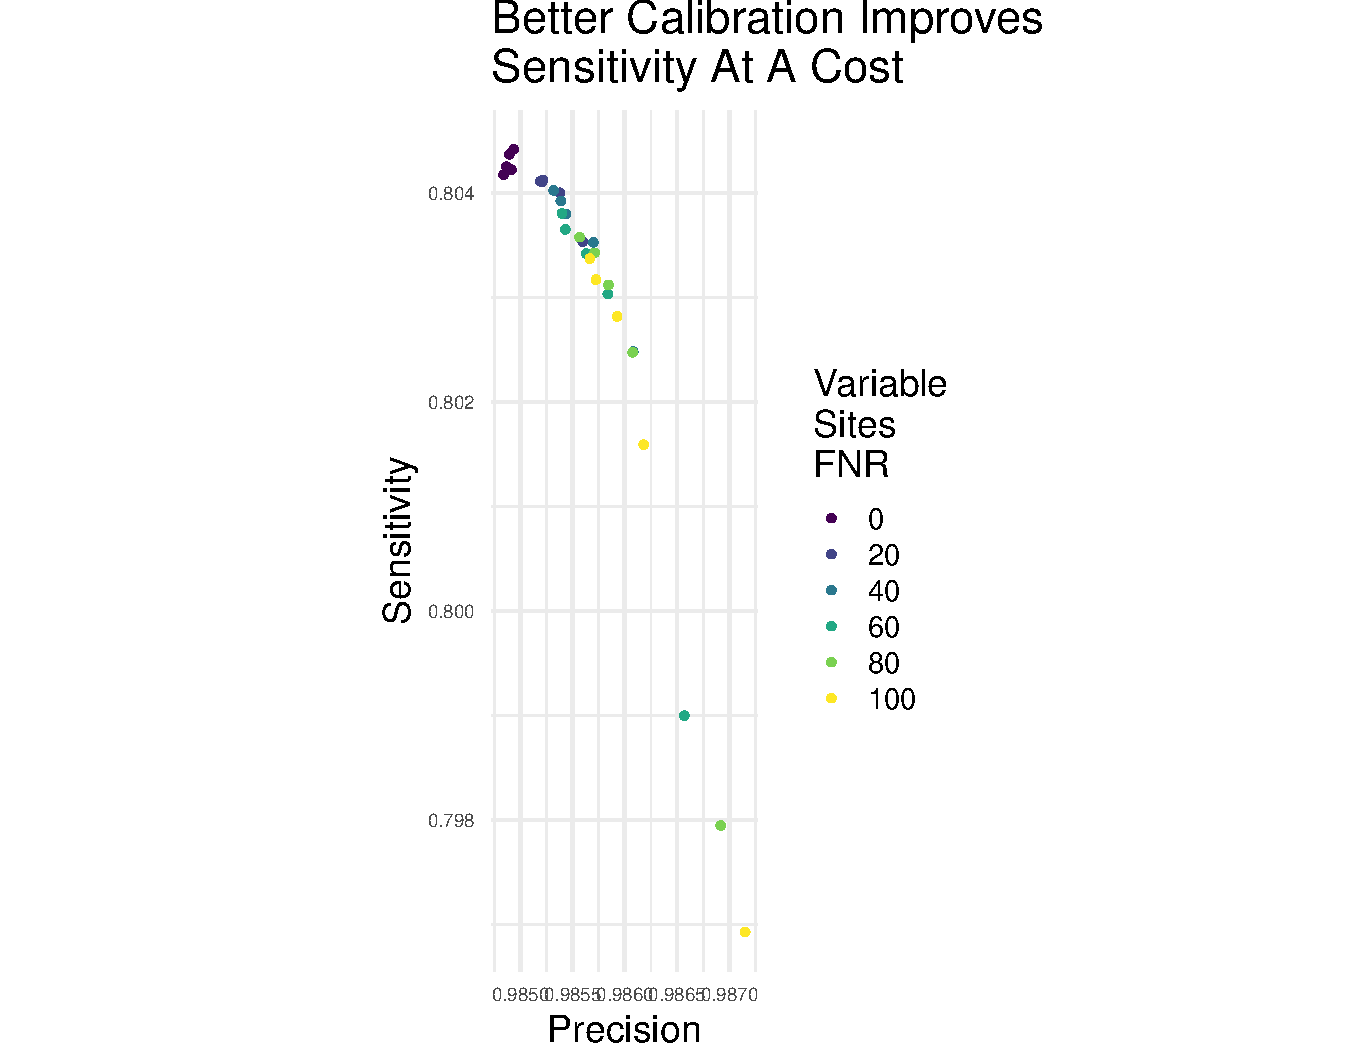
\includegraphics[width=.7\linewidth]{flt_sens_precision.pdf}
\titlecaption{Filtered Call Precision and Sensitivity}{Filtering increases overall precision.}
\label{fig:vc_flt_ps}
\end{figure}

\begin{figure}
\centering
\includetwo{flt_f_plot.pdf}{flt_f_heatmap.pdf}
\titlecaption{asddf}{asdsad}
\label{fig:vc_flt_f}
\end{figure}


%TODO: fix figure sizes and title line breaks. combine similar plots into 1 figure to make the whole chapter more readable


\section{Discussion}
\begin{outline}
\item As the quality of the calibration increases, the quality of the variant calls also slightly increases.
\item Variant filtering is a common and important step in the variant calling process; variant callers are usually tuned to be very sensitive but not very specific, so most people will do some type of filtering on the output. The most common filter is a depth filter, so I filtered on depths that are unexpectedly large or small. These may signify alignment errors or some other type of oddity that makes the calls less trustworthy.
\end{outline}

\section{Conclusion}
\begin{outline}
\item Quality scores have a limited effect on the variants called
\item Excessive binning removes quality score information and makes it difficult to call variants
\item Use

\end{outline}

\printbibliography
\end{document}

